\documentclass[AMA,STIX1COL]{WileyNJD-v2}

\articletype{Article Type}%

\received{01 June 2018}
\revised{01 August 2018}
\accepted{01 August 2018}

\raggedbottom
\usepackage{subcaption}
\captionsetup[subfigure]{font=normalsize}
\usepackage{matlab-prettifier}
\usepackage{amsmath, amsfonts, amssymb}

\usepackage{glossaries}
\makeglossaries

\begin{document}

\title{Open-source platforms for fast room acoustic simulations in complex structures}
%\title{This is the sample article title\protect\thanks{This is an example for title footnote.}}

\author[1]{Matthieu Aussal}

\author[2]{Robin Gueguen}



%\author[3]{Author Three}

\authormark{AUSSAL \& GUEGUEN}

\address[1]{\orgdiv{Centre de math\'ematique appliqu\'ees}, \orgname{\'Ecole Polytechnique}, \orgaddress{91128 Palaiseau, \country{France}}}

\address[2]{\orgdiv{Institut des Sciences du Calcul et des Donn\'ees}, \orgname{Sorbonne Universit\'e}, \orgaddress{Campus Pierre et Marie Curie - 4 place Jussieu, 75252 Paris Cedex 05 \country{France}}}




\corres{ \email{matthieu.aussal@polytechnique.edu}\\\email{gueguen.robin@gmail.com}}

%\presentaddress{This is sample for present address text this is sample for present address text}

\abstract[Summary]{
This article presents new numerical simulation tools, both for Matlab and \textit{Blender} CAD software. Available in open-source under GPL 3.0 license, it uses a ray tracing / image-sources hybrid method to calculate room acoustics for large meshes. Performances are optimized to solve significant size numerical problems (typically more than 100,000 surface elements and about a million of \textit{rays}). For this purpose, a \textit{Divide and Conquer} approach with a recursive octree structure has been implemented to reduce the quadratic complexity of the ray/element interactions to near-linear. Thus, execution times are less sensitive to mesh density, which allows complex geometry simulations. After ray propagation, a hybrid method leads to image-sources format, which can be visually analyzed to localize sound map. Finally, impulse responses are constructed from the image-sources and FIR filters are proposed natively over 8 octave bands, taking into account material absorption properties and propagation medium. This algorithm is validated by various comparison with theoretical test cases. Furthermore, an exemple on a complex case with the ancient theater of Orange is presented. 
}

\keywords{room acoustic, ray-tracing, image-sources, octree, Matlab, \textit{Blender}, archeology, open-source}

\jnlcitation{\cname{%
\author{M. Aussal}, and
\author{R. Gueguen}, 
} (\cyear{2018}), 
\ctitle{Room acoustic measurement tool for complex geometry}, \cjournal{International Journal for Numerical Methods in Engineering}, \cvol{2018;00:1--6}.}

\maketitle

%\footnotetext{\textbf{Abbreviations:} ANA, anti-nuclear antibodies; APC, antigen-presenting cells; IRF, interferon regulatory factor}

% glossaire
%\section{Glossary\label{app1}}
%\newacronym{CAD}{CAD}{Computer-Aided Design}
%\newacronym{rir}{RIR}{\emph{Room Impulse response}}
%\newacronym{RT60}{$RT_{60}$}{\emph{Reveberation Time at $-60dB$}}
%\newacronym{orchestra}{\textit{orchestra}}{\emph{Semicircular (Roman) or circular (Greek) space between the stage and the first tier}}
%
%CAD}\\
%rir}\\
%RT60}\\
%orchestra} 

\section*{Introduction}
\label{sec1}
Today, digital technologies allow research to explore previously inaccessible areas, as virtual reality for archaeology. In this domain, many works focus on the visual restitution, but acoustic studies can reinforce researches to improve the understanding of the ancient world. For example, during the Roman Empire, architects have designed buildings also based on the sound propagation they wanted to achieve\cite{vitruve}. In this study, we focus on the ancient theater of Orange which has a significant size (100m wide), a complex geometry (ornements, bleachers, columns, arches, etc.) and which is open-air. In a previous work, a complete mesh was designed using \textit{Blender} CAD software \cite{doc_blender}, according to the most recent archeological knowledge \cite{theseRobin}. To be representative, this mesh has hundreds of thousands of elements (triangular faces), with complex shape (see fig. \ref{maillage}). As this numerical model is now used by researchers to perform archeological hypothesis, we developed our own room acoustic software, directly integrated in the archeologists workflow. As the mesh size makes difficult the use of precise methods (FEM, BEM, ...), this software is based on a ray-tracing approximation, in order to compute fastly the full-band room impulse response (50 to 15000Hz). This tool has been developed following two steps. We first build a prototype using \textit{Gypsilab}, an open source Matlab framework for fast prototyping \cite{gypsilab}. This preliminary work was usefull to construct and validate ideas and algorithms. It conducts to the creation of a new toolbox, \textit{openRay}, now added to the master branch of \textit{Gypsilab} and freely downloadable \cite{githubGypsi}. In a second step, all algorithms were retranscrypted in C++ using Qt Creator, leading to an autonomous library \textit{Just4RIR}. A python interface was added, in order to use this library as a \textit{Blender} plug'in. At the end, this plug'in allow archeologists to only work on \textit{Blender}, modifying easily meshes and materials, run acoustic simulation and visualize results. \\
After reminders on acoustical energy propagation represented by ray-tracing, this paper gives implementation details for fast computation for large meshes. At the end, validation test cases are given and application on our modelization of the ancient theater of Orange is performed. 

\begin{figure}[t]
\centering
	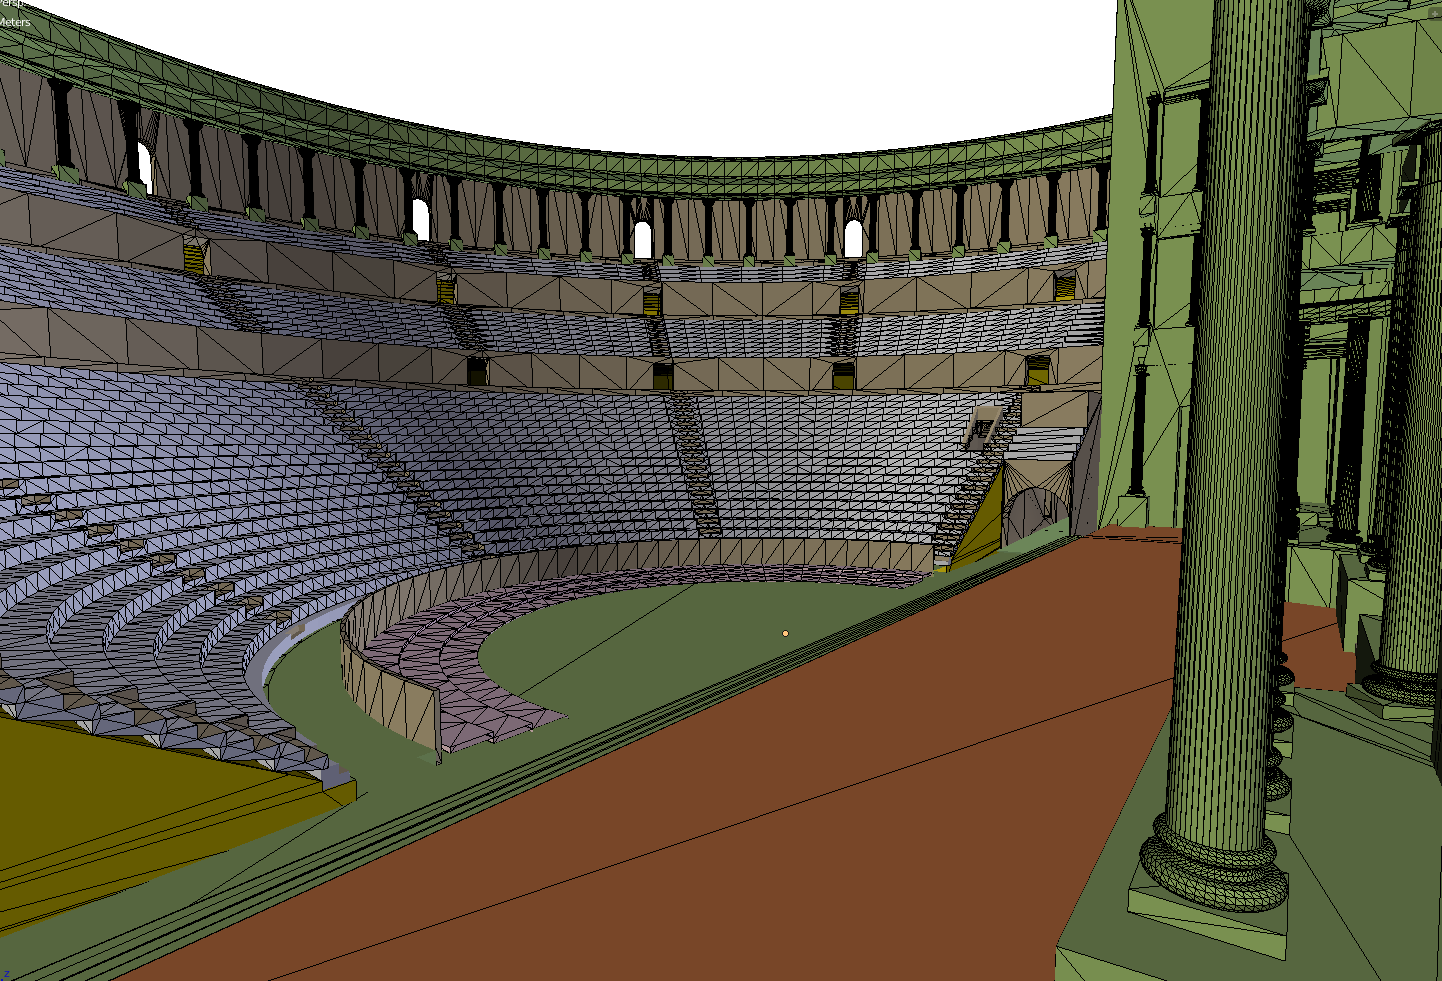
\includegraphics[width=0.5\linewidth]{maillage}
	\caption{Mesh of restituted theater of Orange modelized on \textit{Blender} (436~000 triangles).}
	\label{maillage}
\end{figure}



\section{Acoustical energy modelization}\label{sec2}
\subsection{Continuous domain equation}

By modelling a point sound source as a localized pulse in space, the associated acoustical energy E(t) propagates \cite{jouhaneau} over time on a spherical surface $S(t)$, such that :
%
\begin{equation} 
E(t) = E_0 \int_{S(t)} \overrightarrow{I}(t).\overrightarrow{ds} \qquad \forall t > 0,
\end{equation}
%
with $E_0$ the initial energy and $\overrightarrow{I}(t)$ the acoustical intensity. According to the first principle of thermodynamics and by neglecting the effects of losses related to the absorption of the propagation medium, the acoustic energy is preserved over time. Thus, for a normalized punctual source :
%
\begin{equation} 
\int_{S(t)} \overrightarrow{I}(t).\overrightarrow{ds} = 1 \qquad \forall t > 0.
\label{eq_2}
\end{equation}
%
After integration on the spherical surface $S(t)$, the infinitesimal acoustic intensity is written :
\begin{align} 
% \overrightarrow{I}(t) &= \frac{ \overrightarrow{d}(t)}{4\pi d(t)^3} \qquad \forall t > 0 \nonumber, \\
|| \overrightarrow{I}(t) || &= \frac{1}{4\pi d(t)^2} \qquad \forall t > 0,
\end{align}
%
reflecting that intensity decreases as the square of the distance to the source d(t). Integrating on a portion $\sigma(t)$ of the complete sphere $S(t)$, the energy is then carried by the solid angle $\Omega_{\sigma}$ :
%
\begin{equation}
E_{\sigma}(t) = E_0 \int_{\sigma(t)}  \frac{1}{4\pi  d(t)^2} ds = \frac{E_0}{4\pi}  \Omega_{\sigma}.
\label{eq_4}
\end{equation}
%
This last equation shows that the energy of a solid angle is constant over time and corresponds to a portion of the initial energy~$E_0$. Thus, subdividing $S(t)$ in $N$ portions $\sigma_i(t)$, the total energy can be decomposed as a sum of elementary energies, carried by solid angles $\Omega_i$, such as : 
%
\begin{equation}
E(t) = \sum_{i=1}^N E_i(t) = \frac{E_0}{4\pi}  \sum_{i=1}^N \Omega_i  \qquad \forall t > 0.
\label{eq_5}
\end{equation}
Ones can notice that $(\Omega_i)_{i\in[1,N] }$ is a directional basis, representing energy propagation by piecewise constant elements. Furthermore, for greater clarity, we definitively set in the following $E_0 = 1$.

\subsection{Discrete model}

To numerically represent the energy propagation, we have to discretize basis $(\Omega_i)_{i\in[1,N] }$ in (eq.~\ref{eq_5}). For this purpose, we define a \textit{ray} object composed by :
\begin{itemize}
\item An origin coordinate $x_i$,
\item A direction vector $\overrightarrow{u_i}$,
\item An energy value $E_i$.
\end{itemize}

For example, with an omnidirectional source \footnote{For a directional source, a non-uniform spatial sampling may be used.}, \textit{rays} are given by :
\begin{itemize}
\item The source coordinate ($x_i = x_s,~\forall i\in[1,N]$),
\item A unit sphere uniform sampling (e.g.~icosahedre subdivision, Fibonacci's rule \cite{fibonacci}, etc.),
\item An uniform energy repartition ($E_i = \frac{4\pi}{N},~\forall i\in[1,N]$).
\end{itemize}

To complete this approach, we have to define a discrete measure of energy propagation. To this end, we consider a $r$-radius measurement sphere $S(x_m, r)$, centered on $x_m$.  We can then add the contributions of a $n$-\textit{rays}  beam that intersect this sphere to calculate the acoustic energy $E_m$ at point $x_m$ :

\begin{equation}
E_m \approx  \frac{1}{4\pi}  \sum_{i=1}^n E_i.
\end{equation}
In the particular case of an omnidirectionnal source, we have : 
\begin{equation}
E_m \approx  \frac{n}{N},
\label{eq_7}
\end{equation}
which means that the measured energy $E_m$ is statistically represented by the ratio between the number of \textit{rays} forming a beam to the total number of \textit{rays}.

\begin{figure}[t]
\centering
	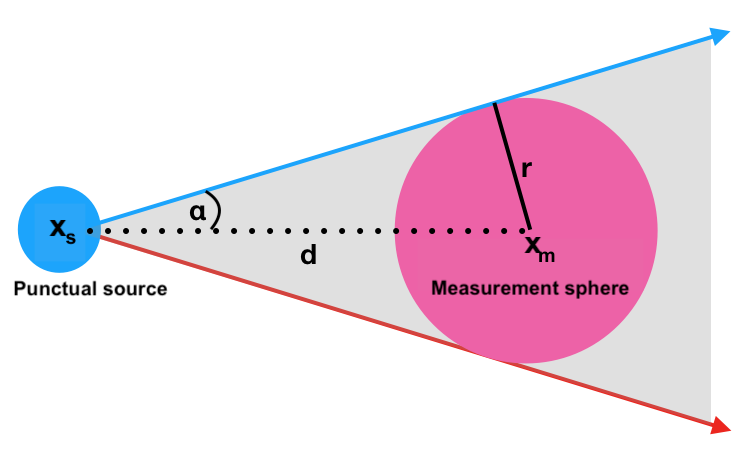
\includegraphics[width=0.6\linewidth]{schema_rayon}
	\caption{Representation of a $r$-radius measurement sphere centered in $x_m$, receiving energy from a sound source in $x_s$.}
	\label{schema_rayon}
\end{figure}

Moreover, applying the continuous model (eq.~\ref{eq_4}), the measured energy is given by :
\begin{equation}
E_m = \frac{1}{4\pi}  \Omega_m,
\end{equation}
where $\Omega_m$ is a solid angle of a cone of revolution (see fig. \ref{schema_rayon}), such as :
\begin{equation}
\Omega_m = 2\pi(1-\cos{\alpha}).
\end{equation}
Following the figure \ref{schema_rayon} :
\begin{equation}
\Omega_m = 2\pi \left( 1 - \sqrt{1-\frac{r^2}{d^2}} \right)
\end{equation}
and considering $\frac{r}{d} \ll 1$, 
\begin{equation}
\Omega_m = \pi \frac{r^2}{d^2}.
\end{equation}
At the end, 
\begin{equation}
E_m \approx  \frac{n}{N} \approx  \frac{\pi r^2}{4\pi d^2}.
\label{eq_12}
\end{equation}
To ensure the existence of this last approximation, beam has to be measurable and count at least one \textit{ray} ($n\geq1$). Thus, fixing a measurement radius r, approximation (\ref{eq_12}) gives a maximum validity range of the discrete model :  
\begin{equation}
\label{eq_13}
	d \leq \frac{r}{2}\sqrt{\frac{N}{n}}.
\end{equation}
In addition, figure \ref{energie} shows how this modelization fills with distance between source and measures. The accuracy of the measurement depends strongly on the number of  \textit{rays} counted, then, the more $n$ increases, the more accurate will be the measurement. Nevertheless, in practice, values for a short distance between the source and the measurement sphere represent direct sound and first reflections, whereas long distances describe the diffuse field. Under this assumption, we can consider this model acceptable for all beam such as $n\geq1$. 

\begin{figure}[t]
\centering
	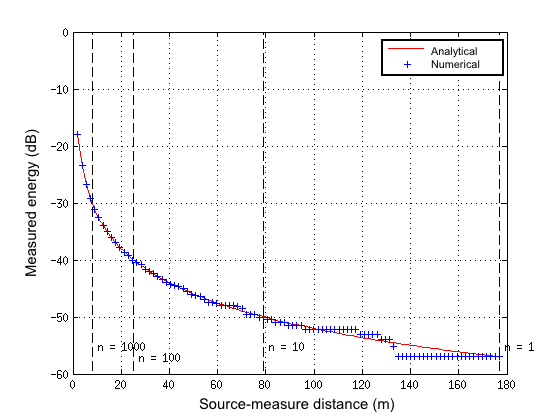
\includegraphics[width=0.65\linewidth]{energie.png}
	\caption{Measured energy (dB) in function of distance between $x_s$ and $x_m$ in meter for $r = 0.36$m and $N = 10^6$. Blue crosses stand for the statistical measure $f(r) = \frac{n(r)}{N}$ and red ligne the analytic function $f(r) = \frac{\pi r^2}{4\pi d^2}$. (computed on \textit{Gypsilab})}
	\label{energie}
\end{figure}

%
\begin{figure}[t]
	\centering
	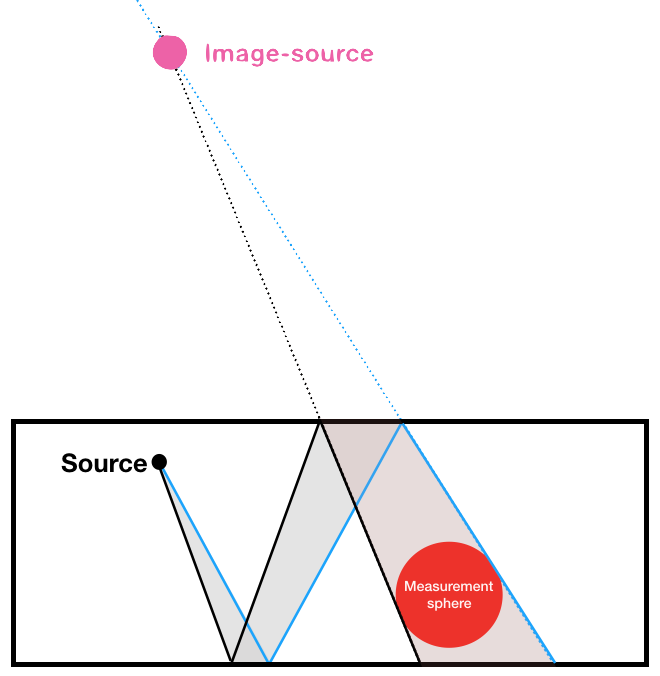
\includegraphics[width=0.5\linewidth]{schema_SI}
	\caption{Sketch of the creation of an image-source by successive reflections of a ray on the walls of a room.}
	\label{schema_SI}
\end{figure}
%Example for bibliography citations cite\cite{Taylor1937}, cites\cite{Knupp1999,Kamm2000}



\subsection{Presence of an obstacle}
For the case of acoustic propagation in presence of an obstacle, we choose to only consider specular reflections (Snell-Descartes laws). Indeed, this approximation is suitable when surfaces are large in comparaison to wavelengths, because diffraction effects can be neglected \cite{jouhaneau}. For a room, this condition is reached if :
\begin{equation}
ka \gg 1, 
\end{equation}
with $k$ the wave number and $a$ the characteristical diameter of the room \cite{hautes_freq}. This approach is currently used by room acoustic softwares (e.g. \textit{Odeon} \cite{odeon}, \textit{Grasshopper} \cite{grasshopper}, etc.) regarding to audible frequency range (62,5 to 15000Hz). In particular, as the theater of Orange has a characteristical diameter about 50 meters, the high frequency approximation is reached. 

Following the discrete model, when an incident \textit{ray} collides a flat surface, a reflected \textit{ray} is generated from the collision point. Noting $\overrightarrow{u_i}$ the direction vector of the incident  \textit{ray}, the reflected direction vector $\overrightarrow{u_r}$ is defined by :
\begin{equation}
\label{eq_15}
\overrightarrow{u_r} = (\overrightarrow{u_i} \cdot \overrightarrow{T})\overrightarrow{T} - (\overrightarrow{u_i} \cdot \overrightarrow{n})\overrightarrow{n},
\end{equation}
with $\overrightarrow{T}$ the tangent basis and $\overrightarrow{n}$ the normal vector of the surface. Moreover, the energy of the reflected \textit{ray} is obtained by :
\begin{equation}
E_r(f) = E_i(f)(1 - \alpha(f)),
\end{equation}
with $\alpha(f)$  the absorption coefficient of the surface, function of the frequency $f$. Practically, the absorption coefficients are often given per octave bands and can be found in various databases. In \textit{Gypsilab} and \textit{Just4RIR}, both use the open access \textit{Odeon} database \cite{odeon} defined on eight octave bands (see table \ref{tab_coeff_abs}). 

Finally, considering wall absorption, energy measured statistically (eq. \ref{eq_12}) is extended by :
\begin{equation}
E_m(f) \approx  \frac{n}{N}(1 - \alpha(f)),
\end{equation}
generalizable to :
\begin{equation}
E_m(f) \approx  \frac{n}{N}\prod_{j=1}^{m}(1 - \alpha_j(f)),
\label{eq_18}
\end{equation}
in the case of $m$ reflexions.

\begin{table}[t]
%\footnotesize
\centering
	\begin{tabular}{| c | m{2.5cm} | *{8}{c|}}
		\hline
		Reference & Material name & 62,5Hz & 125Hz & 250Hz & 500Hz & 1kHz & 2kHz & 4kHz & 8kHz \\
		  \hline
		  \hline
		   1 & 100\% absorbent & 1 & 1 & 1 & 1 & 1 & 1 & 1 & 1 \\
		   \hline
		2 & 100\% reflecting & 0 & 0 & 0 & 0 & 0 & 0 & 0 & 0 \\
		   \hline
		107 & Concrete block, coarse\footnotemark & 0.36 & 0.36 & 0.44 & 0.31 & 0.29 & 0.39 & 0.25 & 0.25 \\
		   \hline
		3000 & Hollow wooden podium\footnotemark & 0.4 & 0.4 & 0.3 & 0.2 & 0.17 & 0.15 & 0.1 & 0.1 \\
	     \hline
	 \end{tabular}
	\caption{Examples of absorption coefficient given in the onligne \textit{Odeon} database \cite{odeon}.}
	 \label{tab_coeff_abs}
\end{table}
\addtocounter{footnote}{-1}
\footnotetext{Harris, 1991}
\addtocounter{footnote}{1}
\footnotetext{Dalenback, CATT}


\subsection{Image-sources}
\label{is}
Although the extended formulation (eq. \ref{eq_18}) may be sufficient to generate room acoustic data, we also construct images-sources from the path of \textit{rays}. To this end, when \textit{rays} intersect a measurement sphere and following the reverse return principle, they are retro-propagated along the last direction vector. Thus, from this measurement sphere, \textit{rays} focus on punctual images-sources (see fig. \ref{schema_SI}). Each image-source is then located relatively to the listener and carry an energy according to equation (\ref{eq_18}). By noting $(x_s)_{s \in [1, N_s]}$ the relative position of the $N_s$ image sources and $(E_s)_{s \in [1, N_s]}$ the associated energy, couples $(x_s;E_s(f))_{s \in [1, N_s]}$ contain many useful informations for room acoustic analysis and auralization. 

First of all, relative distance of each source image $(d_s)_{s \in [1, N_s]}$ can be computed. This distances should be used to compute air absorption, adding a term in the equation (\ref{eq_18}) :
\begin{equation}
E_s(f) \approx  \frac{n}{N}  e^{-\beta(f) d_s}  \prod_{j=1}^{m}(1 - \alpha_j(f)),
\label{eq_19}
\end{equation}    
with $\beta(f)$ a frequency dependent coefficient (ref norme). Furthermore, fixing the sound celerity $c$, room impulse response can be generated, converting each distances $d_s$ in time of arrival. Taking care to convert energy into sound pressure ($p = \sqrt{E}$), finite impulse response can be generated and analyzed using standard metrics (e.g. $T_{30}$, $C_{80}$, $D_{50}$, etc.). For auralization, this room impulse response is convolved with an audio signal in order to listen the acoustical rendering. In particular, this convolution can involve relative position of predominant images sources, in order to realize a spatialized auralization with multichannel or binaural renderers. Finally, to complete acoustic studies with visual analysis, images sources can be projected on the room used for computation to see where are located listened reflections (see last impact on fig. \ref{schema_SI}).



\section{Implementation}
\subsection{Standard algorithm}
As standard principles are introduced, we focus now on the numerical implementation of an acoustic renderer by ray-tracing. Before any acoustic computation, a numerical room has to be modelized with surfaces and materials. In our case, we use simplex representation with meshes composed of flat triangles. From it, geometrical intersection are computed between \textit{rays} (represented by oriented line $(L)$) and mesh elements (represented by piece of plan $(P)$), using parametric equations :
\begin{eqnarray}
(L) &:& a + \delta \overrightarrow{u}, \quad \delta \in \mathbb{R},  \\
(P) &:& b + \lambda \overrightarrow{v} + \mu \overrightarrow{w}, \quad \lambda, \mu \in \mathbb{R}.
\label{eq_20}
\end{eqnarray}    
The following conditions determine pairs (\textit{rays};elements)  with unicity : 
\begin{itemize}
\item $0 < \lambda \leq 1$ and $0 < \mu \leq 1$ to ensure that \textit{ray} is inside the triangle,
\item $\delta > 0$ to respect the propagation direction,
\item $\delta$ minimum not to go throught the mesh.
\end{itemize}
Practically, to find these pairs, we can solve directly underlying linear system with or use the Moller-Trumber algorithm \cite{moller}. For $N$ \textit{rays} and $M$ triangular elements, this process has a numerical cost quadratic proportional to $NM$, which is critical if both $N$ and $M$ are large (see section \ref{octree}). Once all pairs found, energy measurement has to be done in order to build images-sources (see section \ref{is}). To this end, \textit{rays} are intersected to the measurement sphere $S(x_m, r)$ using its cartesian representation :
\begin{equation}
(x-x_m)^2 - r^2 = 0, \quad \forall x \in  \mathbb{R^3},
\end{equation} 
which leads to a linear numerical cost proportional to $N$.

%Finally, while distance travelled of a \textit{ray} verify condition (\ref{eq_13}), it is reflected according to equation (\ref{eq_15}) and propagated. 

Finally, a \textit{ray} is reflected according to equation (\ref{eq_15}) and propagated while its distance travelled verify condition (\ref{eq_13}). This iterative strategy ensure the energy propagation by the elimination of all \textit{rays} that would be in non-measurable beams. In the particular case of an open-air room, \textit{rays} which don't encountered surface of the mesh are also eliminated. Once all \textit{rays} are eliminated, images-sources can be built and post-treated (room impulse response, auralization, etc.).


\subsection{Tree-base acceleration}
\label{octree}
The most critical stage of the standard algorithm is the research of intersections between  \textit{rays} and triangular elements, leading to a quadratic complexity $O(N\times M)$. Indeed, each \textit{ray} has to be tested with each face, for each iteration of the ray-tracing algorithm. For a large number of mesh elements (e.g. $M>10^5$ for the Orange theater) and a lot of \textit{rays} to ensure reasonable accuracy (typically $N>10^6$), the calculation time may be prohibitive. To alleviate this problem, a "Divide and Conquer" approach using binary trees is performed (ref cooley tuckey fft, hierarchical matrix hackbush). The general principle consists in creating a mother-box, containing all the mesh elements. This mother-box is then subdivided along the main dimension to create two daughter-boxes, each with the same number of elements (median spatial subdivision). This process is then applied recursively, until a stopping criterion is reached. In our case, we stop when leaves contain only one element (see fig. \ref{octreeSuzanne}). This hierarchical tree is completely mesh dependent, computed in $O(M\log M)$ operations, and gives a structure to fastly navigate inside the mesh. Thus, at each ray-tracing iteration, rather than face off all \textit{rays} against all elements, this structure is used to accelerate this process. 

\begin{figure}[t]
\centering
		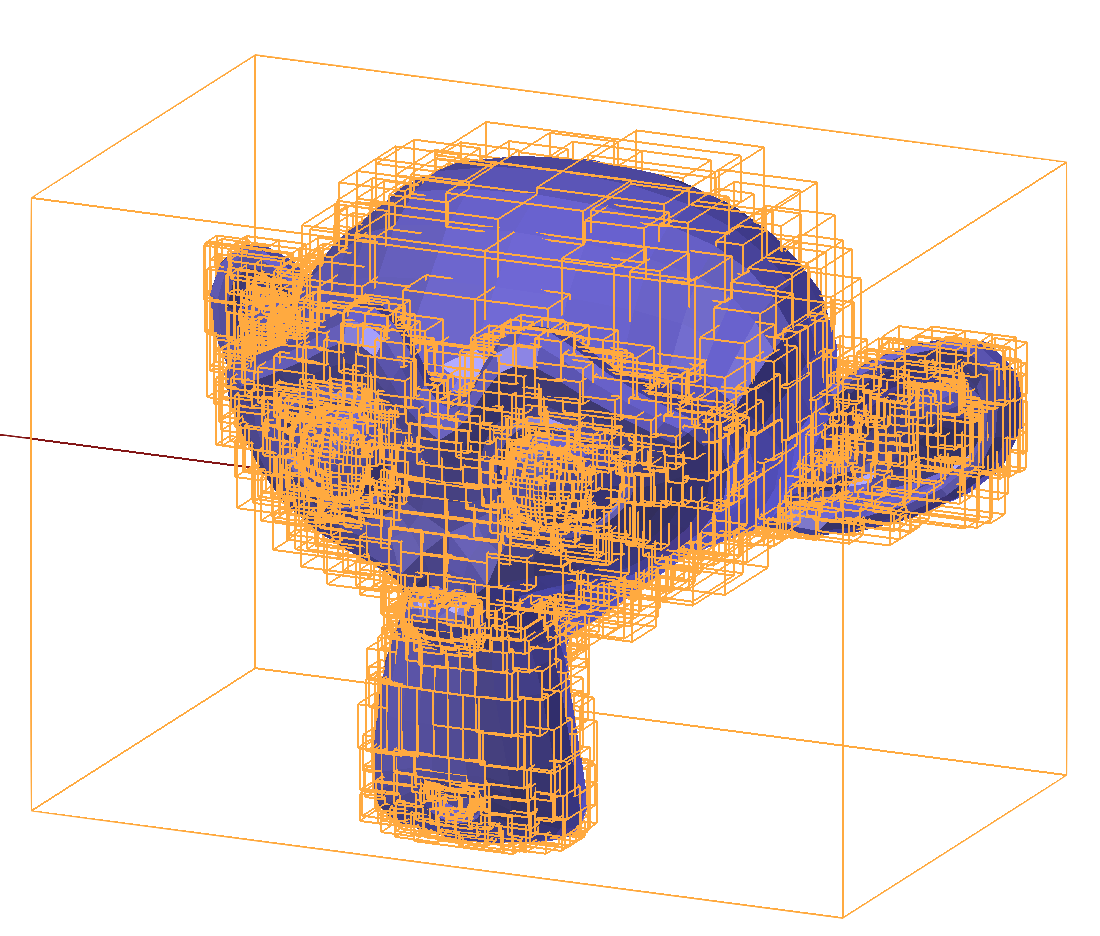
\includegraphics[width=0.4\linewidth]{octreeSuzanne}
		\caption{Binary tree leaves of an arbitrary mesh from \textit{Blender}. (computed on \textit{Just4RIR})}
		\label{octreeSuzanne}
	%\label{octree}
\end{figure}

More precisely, we first initialize the ray-sorting considering a bounding box, containing all \textit{rays} and all elements. After the first median subdivision, we have to distribute \textit{rays} inside the two new boxes. This stage is done in $O(N)$ operations using W.Amy \textit{et al.} algorithm \cite{AABB}. Each box has $N_1$ and $N_2$ \textit{rays}, such as $N = N_1 + N_2$. Assuming this subdivision performed recursively to the $p$-level, each box contains $(N_i)$ \textit{rays} such as: 
\begin{equation}
N = \sum_{i=1}^{2^p} N_i.
\end{equation}  
Then, ray sorting at the $(p+1)$-level also conducts to $O(N)$ operations. To reach the leaves-level, we have to perform $O(N \log M)$ operations, where $\log M$ is close to the depth of the binary tree. At the end, as we have only one element per box, the ray-element intersection only needs $O(N)$ operations. Finally, instead of $O(N M)$ operations, we compute ray-tracing algorithm in~: 
\begin{equation}
O(M\log M) + O(N \log M) + O(N),
\end{equation}  
witch is a quasi-linear complexity. More over, if binary tree is precomputed, each iteration of ray-tracing just stands for :
\begin{equation}
O(N \log M) + O(N).
\end{equation}
 
To evaluate numerically complexities with or without binary tree acceleration, we measure the computation time of one iteration by increasing the number of \textit{rays} and the number of faces in the mesh ($N=M$). As we can see in figure \ref{times}, the complexity of the algorithm is therefor quite linear by using tree-based method. This allows to treat large meshes with millions of \textit{rays}, by maintaining a weak computation time. In particular, we can see in the table \ref{tabComplexite} that for 250~000 \textit{rays} and faces the computation time is divided by a factor of a thousand. It's important to precise that no parallelization strategy has been employed, all results are obtained in single core computation on a standard laptop (2.7 GHz core and 8 Go ram).


\begin{figure}[t]
\centering
	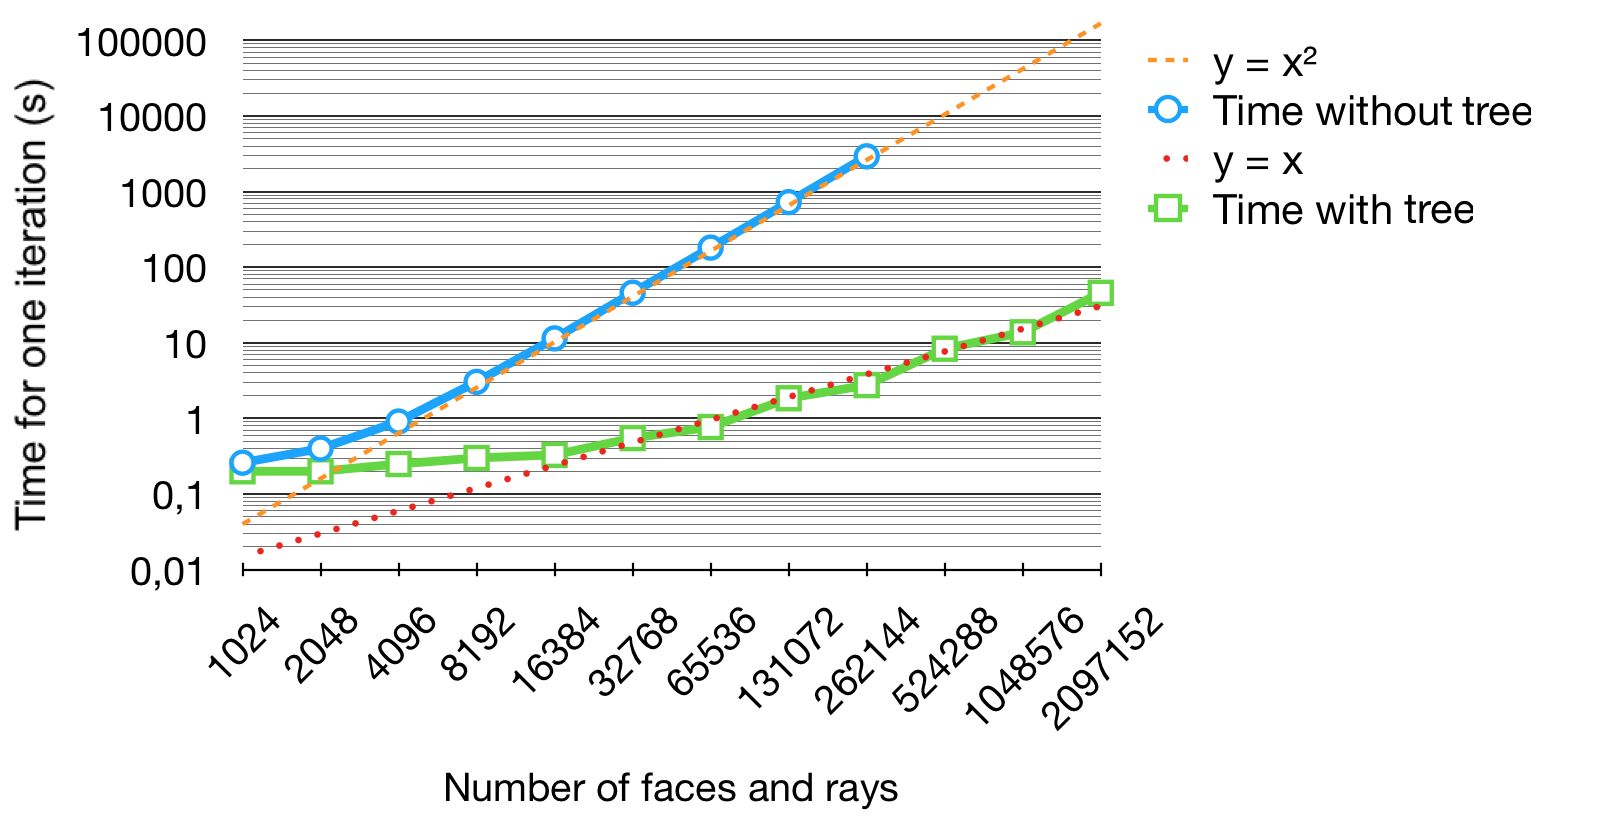
\includegraphics[width=0.8\linewidth]{times}
	\caption{Computation time for one iteration of ray-tracing in function of the number of face and rays, such as $N = M$ (log~scale). An omnidirectional source is located at the center of a mesh of a unitary tetrahedral. (computed on \textit{Just4RIR})}
	\label{times}
\end{figure}
%
\begin{table}[t]
\centering
	\begin{tabular}{| c | c | c |}
		\hline
		Number of faces and \textit{rays} & Time \textbf{without} tree (s) & Time \textbf{with} tree (s)\\
		  \hline
		  \hline
		   $2^{10}$ (=1~024) & 0,26 &	0,2 \\
		   \hline
		$2^{11}$ (=2~048)  & 0,4	& 0,2 \\
		   \hline
		$2^{12}$ (=4~096) & 0,91	& 0,25\\
		   \hline
		$2^{13}$ (=8~192) & 3,05 &	0,3\\
		   \hline
		$2^{14}$ (=16~384) & 11,44	&0,33\\
		   \hline
		$2^{15}$ (=32~768) & 46,02	&0,55 \\
		     \hline
		    $2^{16}$ (=65~536) & 181,61	& 0,77\\
		   \hline
		$2^{17}$ (=131~072) & 725,17	& 1,85\\
		\hline
		$2^{18}$ (=262~144) & 2927,9 & 2,76 \\
		\hline
		$2^{19}$ (=524~288) & X & 8,36 \\
		\hline
		$2^{20}$ (=1~048~576) & X & 13,78 \\
		\hline
		%$2^{21}$ (=2~097~152) & X & 45,83 \\
		%\hline
	 \end{tabular}
	\caption{Computation time of fig. \ref{times} on a standard laptop (2.7 GHz core and 8 Go ram).}
	\label{tabComplexite}
\end{table}



\section{Numerical validation}
To evaluate and validate methods and algorithms, several non-regression tests has been implemented. In this study, we focus only on two examples, that we hope will be the most significant. For more details, readers can refers to R. Gueguen PhD manuscript \cite{theseRobin} or \textit{Gypsilab} source code \cite{githubGypsi}.   

\subsection{Energy conservation by reflecting sphere}
Firstly, we want to prove that statistical approach combined to fast algorithm is able to conserve acoustical energy (eq. \ref{eq_2}). To do this, we consider an academic problem, where the room is a $100\%$ reflecting unit sphere, containing punctual source and measure located at the center. If we consider only specular reflections with no air-absorption, it is expected that energy measurement takes out a Dirac comb, two meters spaced.
Numerically, as we discretize the sphere with flat triangles, this focusing property clearly depend of the mesh refinement. As shown on figure \ref{test2RIR}, numerical diffusion appears in function of the distance.  At the end, only the $10^5$ elements mesh is able to maintain a pulsed energy in the range given, and this computation needs fast methods. Practically, this problem is representative of curved surfaces in rooms, which need high refinement to ensure a good propagation of the acoustic energy.

\begin{figure}[t]
\centering
		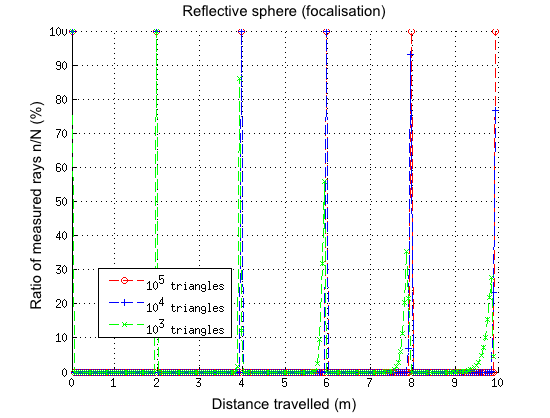
\includegraphics[width=0.6\linewidth]{sphere}
		\caption{Energy measured according to equation \ref{eq_7} for a 100\% reflecting unit sphere, with punctual source and measure located at the center (in percent). This result is given after six iterations of the tree-based algorithm, and we note as expected a two meters distance between pulses. $10^4$ \textit{rays} have been used. (computed on \textit{Gypsilab})}
		\label{test2RIR}
\end{figure}

\subsection{Analytical comparison by shoes box model}
Secondly, numerical computation is compared to the analytical shoes box model, introduced by S. McGovern \textit{et al.} \cite{mcgovern}. This model gives image-sources positions at any reflection order, in function of punctual source and measure located inside a the box. Originally, the energy associated to each image-source is given by :
\begin{itemize}
\item Quadratic decrease $1/d^2$, where d stands for image sources distances to measurement point,  
\item Absorption coefficients $\alpha$ for each wall, with no frequency dependance.
\end{itemize}
To use this model for our validation process, we add to McGovern solutions a frequency dependance for wall absorption, and the atmospherical impact in function of the distance. This extended model gives the energy as equation (\ref{eq_19}), but the statistical counting is there replaced by the distance quadratic decrease.

To compare analytical extended model and numerical ray-tracing computation, we use a simple triangular mesh of $M=12$ triangular elements building a $[5,4,3]$ meters box. A randomly location is given for source ($x_s = [4,2,1.7]$ m) and an arbitrary measurement sphere is fixed ($x_s = [2,2,1.7]$ m and $r=0.2$ m). Wall absorption coefficients are chosen randomly in the Odeon database \cite{odeon}, and atmospheric model is used following the norm ISO-9613-1\cite{iso}. $N = 10^ 5$ rays were used and iterations were stopped according to criterion (\ref{eq_13}). As a results, figure \ref{sourcesImages} show images sources computed which fit exactly to analytic positions (machine accuracy). As tri-dimensional representation is really confusing, we only represent images sources in the plan $z = 1.7$ m. Furthermore, energy value is given in decibel on the color bar, in order to visually see the distance decrease. More precisely, figure \ref{boite} shows a comparison of the energy in decibel, in function of the distance of source images. As expected, a good matching is reached for direct sound and early reflections and diffuse field seems well approached. 
 
\begin{figure}[t]
\centering
	\begin{subfigure}{0.49\textwidth}
		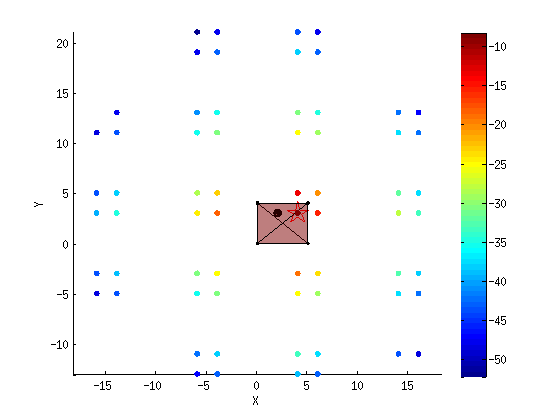
\includegraphics[width=\linewidth]{sourcesImages}
		\caption{Image sources in the plan z = 1.7 m and associated energy (dB). Analytical and numerical solutions are the same, to the precision of the machine.}
		\label{sourcesImages}
	\end{subfigure}
	\begin{subfigure}{0.49\textwidth}
		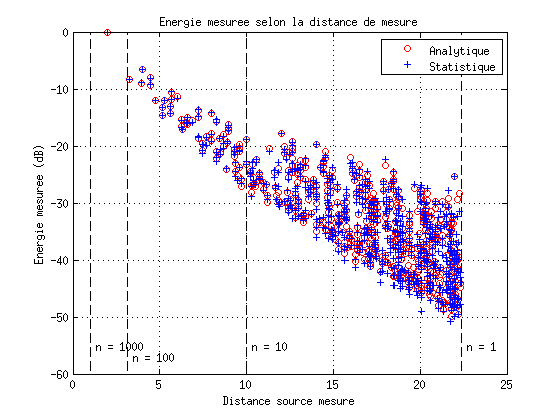
\includegraphics[width=\linewidth]{boite}
		\caption{Energy impulse response in dB. Even if accuracy decreases with the distance, far solutions remain acceptable to describe the diffuse field. }
		\label{boite}
	\end{subfigure}
	\caption{Numerical solutions from ray-tracing inside a shoes box model. Comparisons with analytical solutions. (computed on \textit{Gypsilab})}
\end{figure}


\section{Application to Orange theater}

The fast ray-tracing algorithm allows acoustical computation for complex rooms as the ancient theater of Orange. Indeed, using a virtual model, archeologists can explore many architecture hypothesis. In particular, acoustical analysis allows to understand some behaviors like : the influence of the position of spectators in bleachers, the shape of the roof, the materials of the \textit{orchestra}, etc. Moreover, it is interesting to study where reflections come from, and more generally how the theater responds to acoustical sources in various location.     

First of all, a restituted version of the Orange theater has been meshed on the software \textit{Blender} (fig. \ref{soft}), according to the archeological surveys performed by l'Institut de Recherche sur l'Architecture Antique (IRAA) \cite{orangeTxt}. As this mesh just have to fill the geometry, there is no need of Delaunay properties, but the architecture complexity however conduct to a 436~000 faces triangulation (see fig. \ref{maillage}). In particular, this monument is mainly composed by :
\begin{itemize}
 \item \textit{Postscaenium} (stage wall) partially ornamented with two basilicas on either side,
 \item \textit{Pulpitum} (stage),
 \item \textit{Orchestra},
 \item \textit{Cavea} (bleachers) with \textit{Porticus} at the top (column gallery),
  \item Various covers (stage roof, \textit{velum}, etc.).
\end{itemize}
Several materials are assigned to each part, in order to define specific absorption coefficients taken from Odeon database \cite{odeon} (see fig. \ref{soft}). The ray-tracing solver is then used to compute the spatial impulse response. To reach the reverberation time close to -60dB ($RT_{60}$), we fix one million \textit{rays} and a 2m-radius measurement sphere. The result is obtained in few minutes on a standard laptop (2.7 GHz core and 8 Go ram). At the end, all sources-images positions are generated as well as the associated multi-band acoustical energy (i.e. couple $(x_s;E_s(f))_{s \in [1, N_s]}$, see section \ref{is}). From it, multi-outputs are analyzed in order to study the acoustical behavior of the theater.

The following results are obtained with a source located at the front stage, at 1,60 m high (position of the mouth of an average actor). The listener is on the same axis in the bleachers. On figure \ref{rirTheatre20}, we see the multi-band impulse response of the theater until the maximum distance determined by equation \ref{eq_13}. Primary reflections appear on the first 400 ms and diffuse field decreases according to the frequency. This difference is due to atmospheric absorption and materials properties and only frequencies above 1kHz reach $RT_{60}$. Furthermore, the projected images-sources represented on figure \ref{isTheatre20} illustrate a spatial diffusion. Indeed, even if some areas carries a lot of images-sources, reflections seem to surround the listener. For a better understanding, we zoom on the top of the signal in figure \ref{SItheater} to display energy on a smaller range, which highlight where beams reflect on. We can notice high contribution of the \textit{orchestra}, the wall-stage, the stage and the roof, as F. Canac demonstrated in the 60' \cite{canac}. To finish, perceptive factors were computed from the energy impulse responses, and given in table \ref{tab_rindel}. Results correspond to a room adapted for musical playback (e.g. clarty $C_{80}$ and reverberation time $T_{30}$), more than a speach transmission \cite{acoustique}. This results are confirmed by an equivalent simulation in the Odeon software, using same mesh and parameters.


\begin{figure}[t]
\centering
		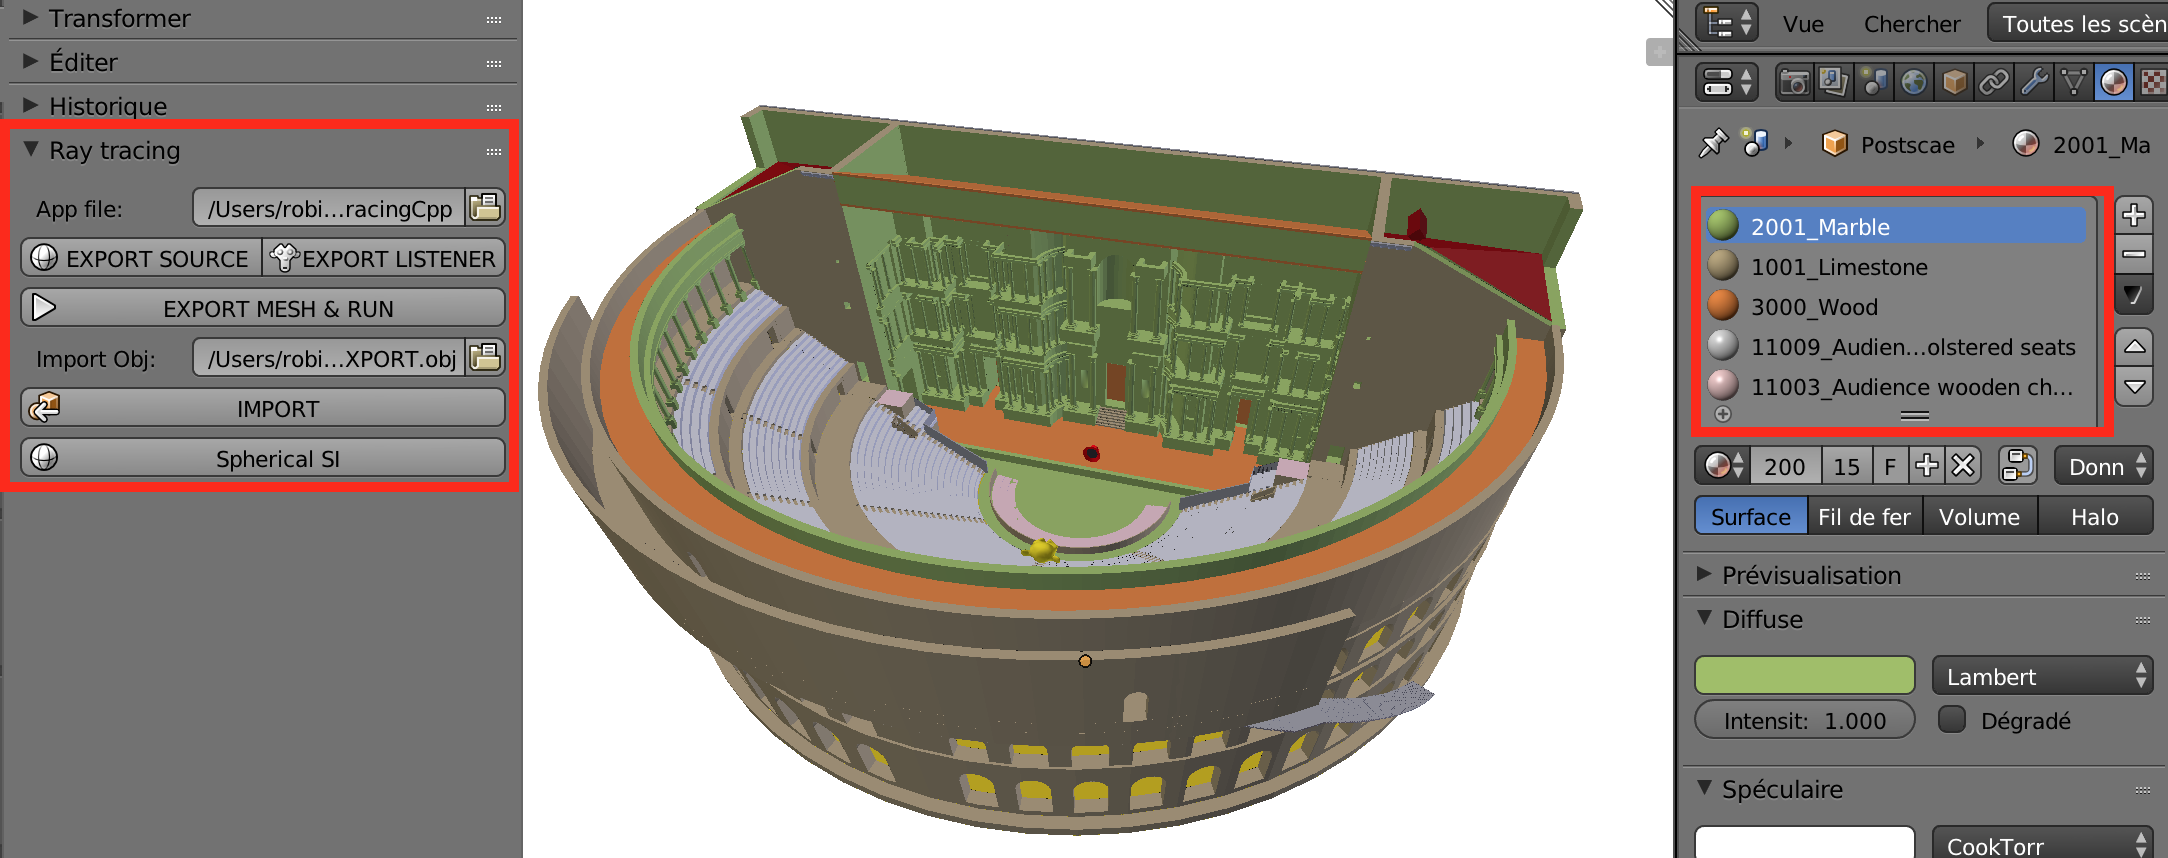
\includegraphics[width=0.9\linewidth]{soft}
		\caption{Modelization of restituted theater of Orange \cite{theseRobin} in \textit{Blender} showing the ray-tracing add-on on the left and the material interface on the right.}
		\label{soft}
\end{figure}


\begin{figure}[t]
\centering
	\begin{subfigure}{0.6\textwidth}
		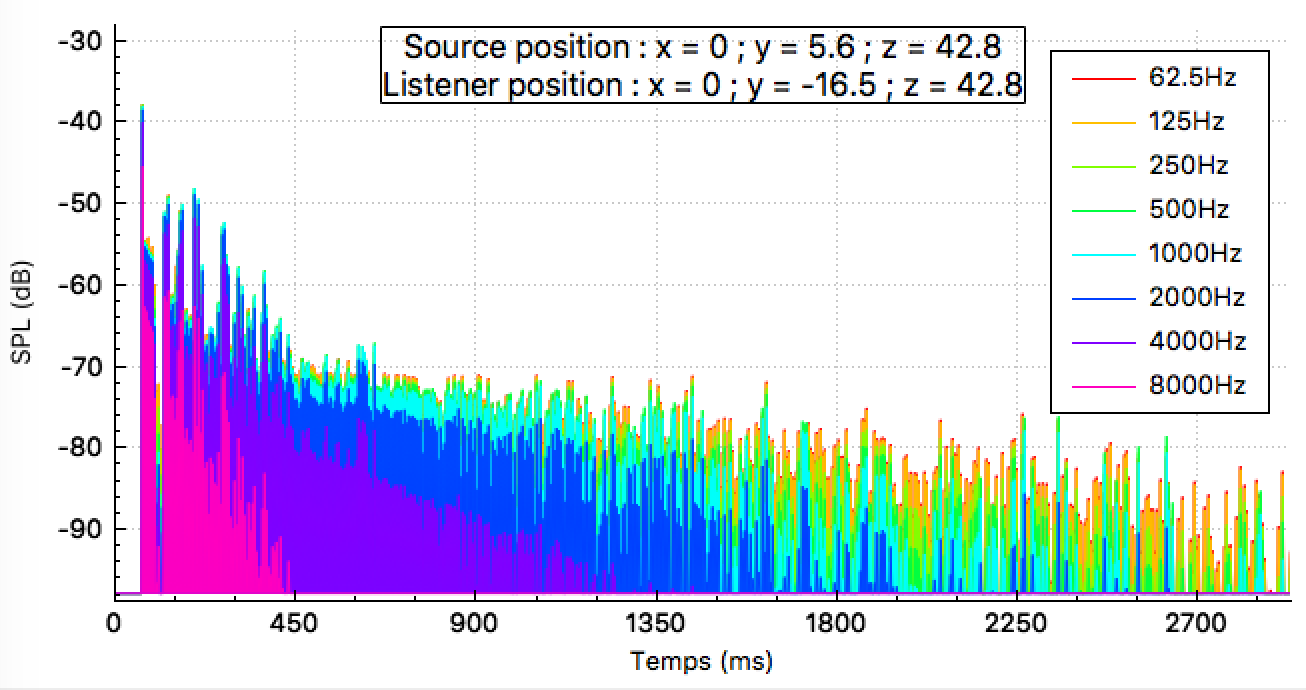
\includegraphics[width=\linewidth]{rirTheatreAvecDecor}
		\caption{Impulse response in dB.}
		\label{rirTheatre20}
	\end{subfigure}
	\begin{subfigure}{0.37\textwidth}
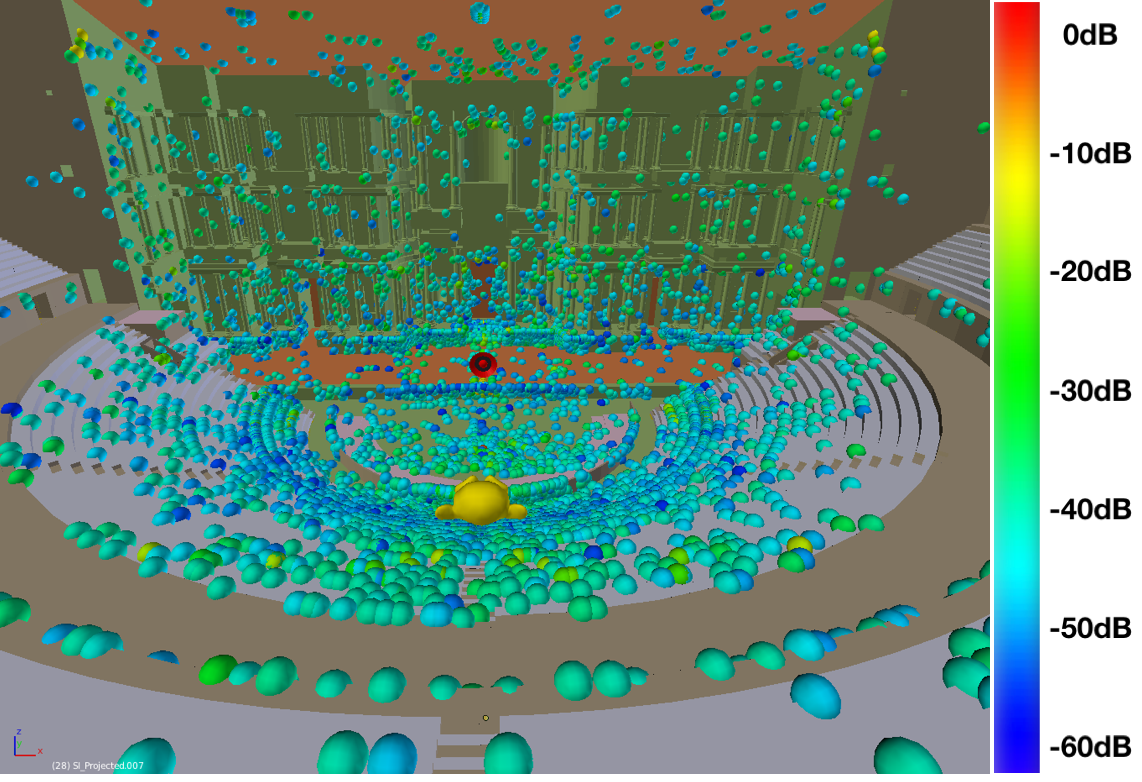
\includegraphics[width=\linewidth]{SI60dB}
		\caption{Images-sources projected on the mesh.}
		\label{isTheatre20}
	\end{subfigure}
	\caption{Ray-tracing outputs for one million \textit{rays} and a 2m-radius sphere (listener) on restituted theater of Orange.  (computed on \textit{Just4RIR})}
	\label{SI60dB}
\end{figure}



\begin{figure}[t]
\centering
	\begin{subfigure}{0.63\textwidth}
		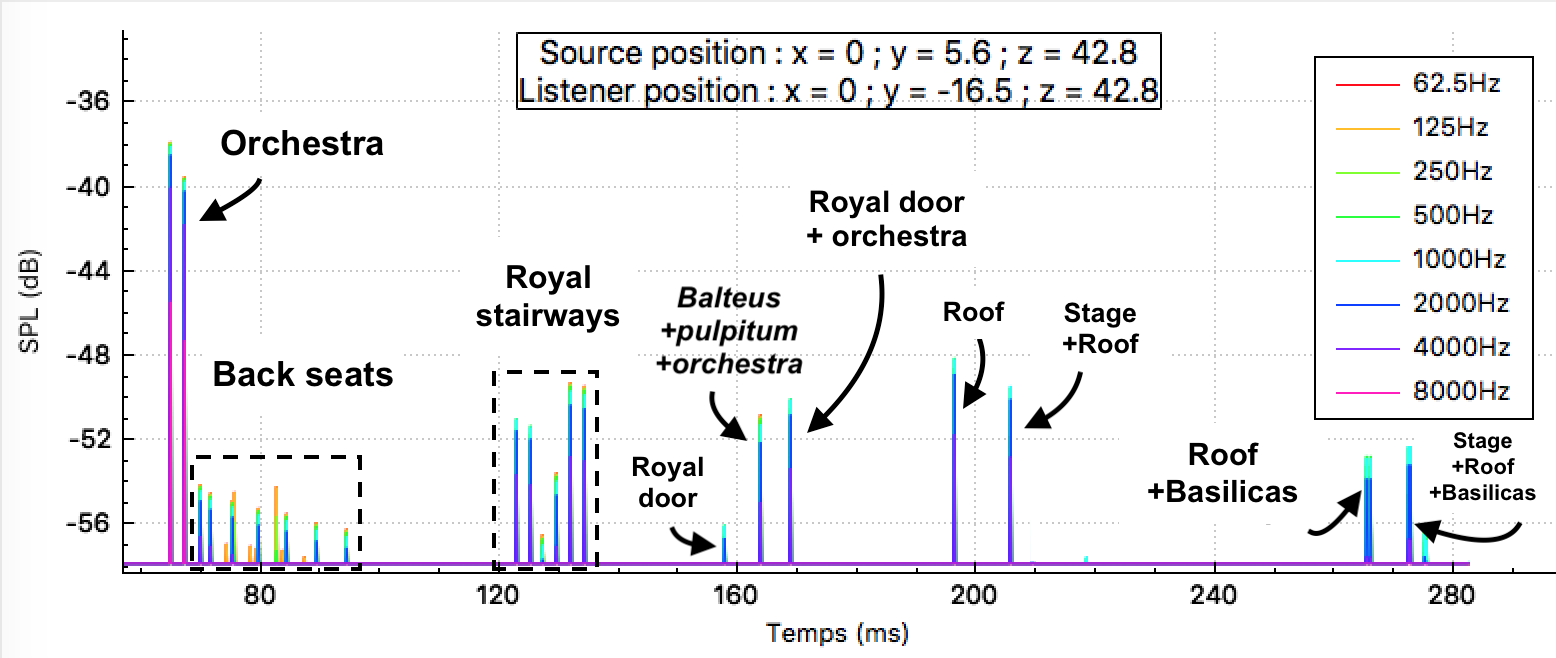
\includegraphics[width=\linewidth]{rirTheatre20}
		\caption{Impulse response of the first reflections over 20dB range.}	
		\label{RIR20dB}
	\end{subfigure}
	\begin{subfigure}{0.36\textwidth}
		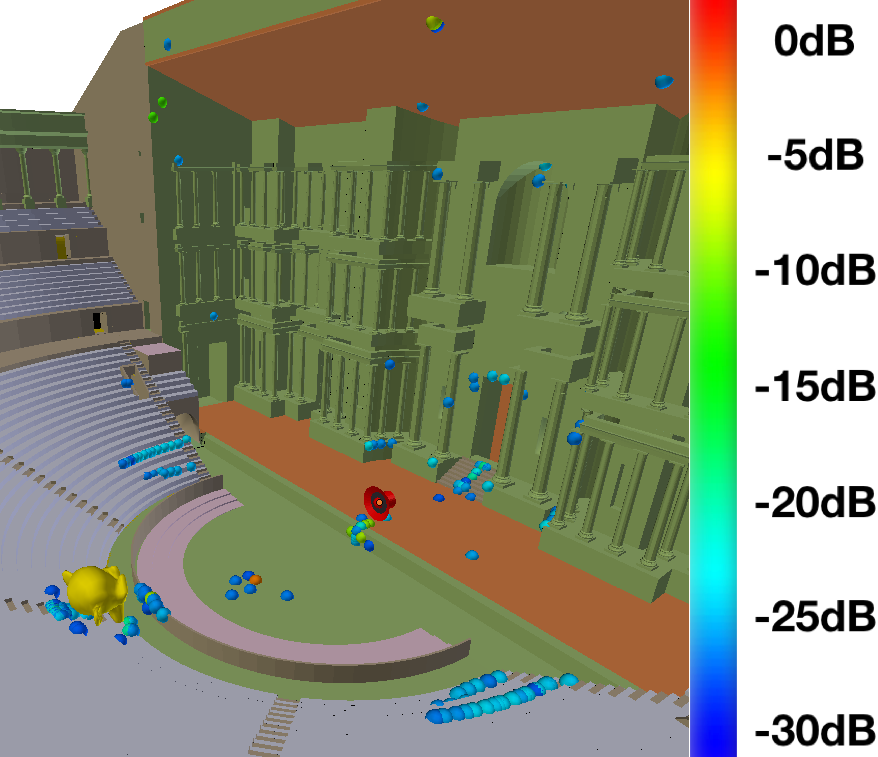
\includegraphics[width=\linewidth]{SI30dB}
		\caption{Images-sources of the first reflections over 30dB range, projected on the mesh.}
		\label{SI30dB}
	\end{subfigure}
	\caption{Zooming on the first reflections of fig. \ref{SI60dB}. (computed on \textit{Just4RIR})}
	\label{SItheater}
\end{figure}

\begin{table}[h]
\centering
 \begin{tabular}{| *{3}{c|}} 
 \hline 
 Perceptive factors & \textit{Just4RIR} & \textit{Odeon} \\ 
 \hline 
 \hline 
  EDT (s)& 1.85& 2.1 \\ 
 \hline 
$T_{30}$ (s)& 3.59&  2.73\\ 
 \hline 
SPL (dB) &-32 & -32.4\\ 
 \hline 
$C_{80}$ (dB)& 1.12&1.5  \\ 
 \hline 
$D_{50}$ (\%)&47 & 52 \\ 
 \hline 
$T_s$ (ms)&117 & 105 \\ 
 \hline 
\end{tabular} 
 \caption{Perceptive factors obtained for the Orange theater, comparison between \textit{Just4RIR} and \textit{Odeon} software \cite{odeon}. The measure is done on the 500-1000Hz band.}
 \label{tab_rindel} 
 \end{table}

\section{Conclusions}

In this paper, a full-chain engineering process is given, leading by an acoustical study of an imposing ancient monument. From archaeological needs, a fine mesh of the monument was constructed, associated to a complete room acoustic application suite, both for Matlab and \textit{Blender}. The high complexity provided by this type of architecture and its ornaments leads to approximate calculation methods. Indeed, by only simulating specular reflections and wall absorption, energy propagation and measurement can be simulated by beams, carried by ray-tracing. From this representation basis, it is possible to generate a multi-band impulse response, while respecting the laws of high-frequency acoustics. Moreover, a fast algorithm with a quasi-linear complexity has been implemented, allowing users to quickly evaluate architectural assumptions, modifying their meshes regardless of the number of elements. At the end, various post-treatment has been added, as the Room Impulse Response generation, the source-image visualization, the classical perceptive factors and an auralization process.

Even if current versions of proposed softwares (Gypsilab \cite{githubGypsi} and \textit{Just4RIR}) are complete enough to be used for various studies, there are many opportunities of improvement. First of all, as image-sources positions are known, a spatial audio renderer should be added to improve current auralization tool (e.g. binaural or multichannel, eventually with trackers). Secondly, as virtual reality is becoming more and more important in today's applications, we could consider moving the listener in real time and thus, allow a complete virtual tour of the building. Finally, as ray-tracing modelization is an high-frequency approximation of waves phenomena, diffraction effects should be added in order to get a better fit with the physics equations. 
%
%We presented the problems raised by an acoustic study of an ancient monument. The complex geometry of this type of building and their colossal size requires the use of approximate calculation methods. Thus, by simulating the reflections and absorptions of the walls, it is possible to study the reverberation of a room. Despite the inevitable approximations of the model, we have proved that the laws of physics are respected. A fast algorithm has been implemented to allow users to easily and quickly test their architectural assumptions. Thus, the calculation time becomes linear to the product number of mesh elements/number of \textit{rays}. The algorithm developed allows the study of the temporal graph of reverberation of the building as well as the position in space of the various sound reflections. Furthermore, a sound signal could be heard in three dimensions thanks to binaural filters and steering control can be done with "Head Tracker" mounted on a headset.
%
%However, there are many opportunities for improvement that remain under consideration for this type of software tool. First, in a context where virtual reality is becoming more and more important in today's applications, we could consider moving the listener in real time and thus, allow a complete virtual tour of the building. Secondly, from the point of view of the analysis results, there are many possible improvements at the graphic level. That raises some questions. How to view acoustic calculation results? What information is essential for an archaeologist wishing to study the acoustics of a monument? Similarly, is it essential to add diffraction effects to the model? If so, what is the best method? Could certain acoustic behaviours be treated locally and then inserted into the model by ray tracing? Finally, it would also be interesting to use sources whose directivity is not uniform. This would be more representative of the real cases, and in particular, of the use made in Orange at the theatre origin. The sounds were then emitted by musical instruments or by the human voice possibly amplified by a mask.

%\subsection{Blender add-on}
%In a second hand the tool is also available as a \textit{Blender} add-on. The user can work on the CAD software to model the room under test, positioning the sources and the receiver and assign materials to the walls. By clicking on the "Run" button, the mesh is exported, the materials are linked to eight absorption coefficients (extracted from a data base) and the acoustic calculation tool is launched. This is an executable C++ complied software which treats information form \textit{Blender} and generates the room impulse response. The communication between the CAD and the executable is done thanks to an .obj file, so using \textit{Blender} is not necessary. Different options allow to analyse the results by reimporting \textit{rays} or image-sources on the CAD software. It is also possible to listen an audio file convolved to the RIR to listen the reverberate sound.
%
%
%\section{Application to the antic theatre of Orange}\label{sec7}
%
%
%The acoustic simulation can be done on the ancient theater of Orange. Because it is an open room the software automatically add a 100\% absorbant box around the building to be sure to always count all \textit{rays}. We can then calculate the image-sources and the RIR for different configurations of the theatre or different materials. Indeed, archeologists want to explore some architecture hypothesis from missing part of the theatre. An acoustical analysis can allow to understand some behaviors like : the influence of the position of the spectators in the bleachers, the shape of the roof, the materials of the \textit{orchestra}, etc. With a 600~000 faces theatre (i.e including decoration elements of the stage wall), the RIR at $RT_{60}$ is generated in 20 minutes for one million \textit{rays} (see fig. \ref{rir}). Each iteration is done in 25s so it really depends on the materials chosen. We can note that the more details of the mesh are refined the more we can simulate diffraction effect. Indeed, in high frequency, small detail elements will be able to reflect the \textit{rays} in different directions which can resemble diffraction effects. In the theater it will be really interesting to study where the reflection come from. Thus, we project the image-sources on the wall of the theater to understand what wall is the main contributor to the energy received (see fig. \ref{theatre}).



\section*{Acknowledgments}
Authors particularly thanks Fran\c{c}ois Alouges, Titien Bartette, Pascal Frey and Emmanuelle Rosso for all the help they each provided at the different stages of this project. Thanks also to Jean-Dominique Polack for advices on architectural acoustics and Martin Lesellier for various contributions. This work is part of R. Gueguen PhD thesis founded by Sorbonne Universit\'e.

\bibliography{Biblio}%

\clearpage

\section*{Annexe}

\begin{lstlisting}[style=Matlab-editor,basicstyle=\footnotesize]

%+========================================================================+
%|                                                                        |
%|            This script uses the \textit{Gypsilab} toolbox for Matlab            |
%|                                                                        |
%| COPYRIGHT : Matthieu Aussal (c) 2017-2018.                             |
%| PROPERTY  : Centre de Mathematiques Appliquees, Ecole polytechnique,   |
%| route de Saclay, 91128 Palaiseau, France. All rights reserved.         |
%| LICENCE   : This program is free software, distributed in the hope that|
%| it will be useful, but WITHOUT ANY WARRANTY. Natively, you can use,    |
%| redistribute and/or modify it under the terms of the GNU General Public|
%| License, as published by the Free Software Foundation (version 3 or    |
%| later,  http://www.gnu.org/licenses). For private use, dual licencing  |
%| is available, please contact us to activate a "pay for remove" option. |
%| CONTACT   : matthieu.aussal@polytechnique.edu                          |
%| WEBSITE   : www.cmap.polytechnique.fr/~aussal/gypsilab                 |
%|                                                                        |
%| Please acknowledge the \textit{Gypsilab} toolbox in programs or publications in |
%| which you use it.                                                      |
%|________________________________________________________________________|
%|   '&`   |                                                              |
%|    #    |   FILE       : nrtRayCube.m                                  |
%|    #    |   VERSION    : 0.41                                          |
%|   _#_   |   AUTHOR(S)  : Matthieu Aussal                               |
%|  ( # )  |   CREATION   : 14.03.2017                                    |
%|  / 0 \  |   LAST MODIF : 01.04.2018                                    |
%| ( === ) |   SYNOPSIS   : Ray tracing with absorbing cube               |
%|  `---'  |                                                              |
%+========================================================================+

% Cleaning
clear all
close all
clc

% Library path
addpath('../../openMsh')
addpath('../../openRay')

% Parameters
L     = [5 4 3]
Xsrc  = [4 2 1.7];
Xmes  = [2 2 1.7];
Nray  = 1e5
rad   = 0.2

% Read mesh
mesh = msh('cube1e1.mesh');

% Mesh reshape to feat dimensions in L
mesh.vtx = 0.5 .* (1 + mesh.vtx);
mesh.vtx = (ones(size(mesh.vtx,1),1)*L) .* mesh.vtx;

% Initialize ray
ray = ray(mesh,Xsrc,Nray);

% Graphical sphere
[X,Y,Z] = sphere(50);
X = Xmes(1) + rad*X; Y = Xmes(2) + rad*Y; Z = Xmes(3) + rad*Z; 

% Graphical representation
figure
plot(mesh)
hold on
surf(X,Y,Z,ones(size(X)))
axis equal;
xlabel('X');   ylabel('Y');   zlabel('Z');
alpha(0.3)
colorbar

% Material properties (http://www.odeon.dk/material-manufactures)
ray.msh.col(mesh.col==1) = 10;    % X = 1
ray.msh.col(mesh.col==2) = 20;    % Y = 1
ray.msh.col(mesh.col==3) = 30;    % X = 0
ray.msh.col(mesh.col==4) = 40;    % Y = 0
ray.msh.col(mesh.col==5) = 50;    % Z = 0
ray.msh.col(mesh.col==6) = 60;    % Z = 1
% ray.msh.col(:) = 60;

% Maximum distances 
r1000 = rad/2 * sqrt(Nray/1000);
r100  = rad/2 * sqrt(Nray/100);
r10   = rad/2 * sqrt(Nray/10);
rMax  = rad/2 * sqrt(Nray/2);

% Ray-tracing
tic
ray = ray.tracer(100,rMax);
toc

% Images sources
tic
[img,nrg] = ray.image(Xmes,rad,rMax);
toc

% Graphical representation for images
n   = size(img,1);
tmp = ones(n,1)*Xmes + img;
tmp = msh(tmp,(1:n)');
plot(tmp,10*log10(nrg(:,1)));
axis equal
colorbar

% Analytical solution
load('odeon.mat')
num = [30 ; % X = 0
    10 ;    % X = 1
    40 ;    % Y = 0
    20 ;    % Y = 1
    50 ;    % Z = 0
    60];    % Z = 1
mat = odeon.mat(num,:);
rhm = 30;
air = 5.5 * (50/rhm) .* (odeon.frq/1000).^1.7 * 1e-4;
tic
[imgRef,nrgRef] = rayCubeAnalytic(L,mat,air,Xsrc,Xmes,rMax);
toc

% Graphical representation
plot3(imgRef(:,1)+Xmes(1),imgRef(:,2)+Xmes(2),imgRef(:,3)+Xmes(3),'ok')

% Data
r    = sqrt(sum(img.^2,2));
rRef = sqrt(sum(imgRef.^2,2));
sol  = mean(nrg,2);
ref  = mean(nrgRef,2);

% Energy error in dB
figure
plot(rRef,10*log10(ref),'or',r,10*log10(sol),'+b')
hold on
plot([r1000 r1000],[-60,0],'k--')
text(r1000,-55,' n = 1000')
plot([r100 r100],[-60,0],'k--')
text(r100,-57,' n = 100')
plot([r10 r10],[-60,0],'k--')
text(r10,-55,' n = 10')
plot([rMax rMax],[-60,0],'k--')
text(rMax,-55,' n = 1')
xlabel('Distance source mesure')
ylabel('Energie mesuree (dB)')
title('Energie mesuree selon la distance de mesure')
legend({'Analytique','Statistique'})
grid on

% Audio file
[audio,fs] = audioread('anechoicVoice.wav');

% Fir from images
T = floor(r/340*fs) + 1;
for i = 1:size(nrg,2)
    fir8(:,i) = accumarray(T,nrg(:,i),[max(T) 1]);
end

% Bank filtering
dir8 = ray.bank(256,fs);
rir  = 0;
abs(sum(sum(dir8,2)) - 1)
for i = 1:size(dir8,2)
    rir = rir + fftfilt(dir8(:,i),fir8(:,i));
end

% Graphical representation
figure
plot(rir)

% Audio rendering (5 seconds)
out = fftfilt(rir,audio(1:5*fs));
sound(out,fs)

disp('~~> Michto \textit{Gypsilab} !')

\end{lstlisting}

%\subsection*{Author contributions}
 

%\subsection*{Financial disclosure}


%\subsection*{Conflict of interest}



%\section*{Supporting information}

%The following supporting information is available as part of the online article:
%
%\noindent
%\textbf{Figure S1.}
%{500{\uns}hPa geopotential anomalies for GC2C calculated against the ERA Interim reanalysis. The period is 1989--2008.}
%
%\noindent
%\textbf{Figure S2.}
%{The SST anomalies for GC2C calculated against the observations (OIsst).}


%\section{Glossary\label{app1}}

%\printglossaries


	

	
		
%Use \verb+\begin{verbatim}...\end{verbatim}+ for program codes without math. Use \verb+\begin{alltt}...\end{alltt}+ for program codes with math. Based on the text provided inside the optional argument of \verb+\begin{code}[Psecode|Listing|Box|Code|+\hfill\break \verb+Specification|Procedure|Sourcecode|Program]...+ \verb+\end{code}+ tag corresponding boxed like floats are generated. Also note that \verb+\begin{code}[Code|Listing]...+ \verb+\end{code}+ tag with either Code or Listing text as optional argument text are set with computer modern typewriter font.  All other code environments are set with normal text font. Refer below example:
%
%\begin{lstlisting}[caption={Descriptive Caption Text},label=DescriptiveLabel]
%for i:=maxint to 0 do
%begin
%{ do nothing }
%end;
%Write('Case insensitive ');
%WritE('Pascal keywords.');
%\end{lstlisting}
%
%
%
%\subsection{Subsection title of first appendix\label{app1.1a}}
%
%\noindent\textbf{Unnumbered figure}
%
%
%\begin{center}
%
\includegraphics[width=7pc,height=8pc,draft]{empty}
%\end{center}
%
%
%%== Figure 4 ==
%%% Example for figure inside appendix
%\begin{figure}[t]
%\centerline{
\includegraphics[height=10pc,width=78mm,draft]{empty}}
%\caption{This is an example for appendix figure.\label{fig5}}
%\end{figure}


%\nocite{*}% Show all bib entries - both cited and uncited; comment this line to view only cited bib entries;


%\section*{Author Biography}

%\begin{biography}{
\includegraphics[width=66pt,height=86pt,draft]{empty}}{\textbf{Author Name.} This is sample author biography text this is sample author biography text this is sample author biography text this is sample author biography text this is sample author biography text this is sample author biography text this is sample author biography text this is sample author biography text this is sample author biography text this is sample author biography text this is sample author biography text this is sample author biography text this is sample author biography text this is sample author biography text this is sample author biography text this is sample author biography text this is sample author biography text this is sample author biography text this is sample author biography text this is sample author biography text this is sample author biography text.}
%\end{biography}

\end{document}
